\documentclass[10pt,twocolumn,letterpaper]{article}

% My own stuff
\usepackage{booktabs}
% \usepackage{caption}
% \captionsetup[table]{skip=8pt}   % Only affects tables
\usepackage{stfloats}  % Add this to the preamble
\usepackage{float}

\usepackage{cvpr}
\usepackage{times}
\usepackage{epsfig}
\usepackage{graphicx}
\usepackage{amsmath}
\usepackage{amssymb}

% Include other packages here, before hyperref.

% If you comment hyperref and then uncomment it, you should delete
% egpaper.aux before re-running latex.  (Or just hit 'q' on the first latex
% run, let it finish, and you should be clear).
\usepackage[breaklinks=true,bookmarks=false]{hyperref}

\cvprfinalcopy % *** Uncomment this line for the final submission

\def\cvprPaperID{****} % *** Enter the CVPR Paper ID here
\def\httilde{\mbox{\tt\raisebox{-.5ex}{\symbol{126}}}}

% Pages are numbered in submission mode, and unnumbered in camera-ready
%\ifcvprfinal\pagestyle{empty}\fi
\setcounter{page}{1}
\begin{document}

%%%%%%%%% TITLE
\title{Parte 1/2 del Resumen Basado en Datos de ECDO: Entendimiento Actual de la Teoría de Oscilación y Desacoplamiento Exotérmico Núcleo-Manto (ECDO) “Vuelco de la Tierra”}

\author{Junho\\
Sitio web: \href{https://sovrynn.github.io}{sovrynn.github.io}\\
Repo de Investigación ECDO: \href{https://github.com/sovrynn/ecdo}{github.com/sovrynn/ecdo}\\
{\tt\small junhobtc@proton.me}
}

\maketitle
%\thispagestyle{empty}

%%%%%%%%% ABSTRACT
\begin{abstract}
En mayo del 2024, un autor en línea con un pseudónimo conocido como “El Escéptico Ético” \cite{0} (The Ethical Skeptic, en inglés) compartió una teoría innovadora llamada la Oscilación del Desacoplamiento Exotérmico Núcleo-Manto Dzhanibekov (ECDO) \cite{1}. Esta teoría sugiere que la Tierra ha experimentado anteriormente cambios súbitos y catastróficos en su eje de rotación, provocando inundaciones enormes en todo el mundo a medida que los océanos se derramaban sobre los continentes debido a la inercia rotacional. Además, presenta un proceso geofísico explicativo y datos que indican que otro cambio de este tipo podría ser inminente. Aunque predicciones de tales inundaciones cataclísmicas y el fin del mundo no son nuevas, la teoría ECDO es singularmente convincente debido a su enfoque científico, moderno, multidisciplinario, y basado en datos.

Este documento es la primera parte de un resúmen de seis meses de investigación independiente en la teoría ECDO condensado en dos partes \cite{2,20}. Destaca tres puntos clave:

\begin{flushleft}
\begin{enumerate}
    \item Un 'vuelco de la Tierra' similar al ECDO ha ocurrido múltiples veces en la historia reciente de la humanidad, como lo evidencian los mitos de inundaciones y las señales geológicas de inundaciones continentales extensas.
    \item La dirección y magnitud aproximada de vuelcos de la Tierra pasados puede ser determinado.
    \item Datos geomagnéticos y geofísicos recientes sugieren que otro vuelco de la Tierra podría ser inminente, y que el cambio climático podría ser causado por cambios profundos dentro de la Tierra, en lugar de por los humanos.
\end{enumerate}
\end{flushleft}

Además, esta teoría cubre la física causal detrás de un “vuelco de la Tierra” propuesto por la teoría ECDO.

En este documento, me mantengo objetivo al centrarme en datos duros, evito las partes de la teoría que son convincentes pero especulativas, y enfatizo que este es un tema que la humanidad tiene una necesidad urgente de investigar más a fondo.
\end{abstract}

%%%%%%%%% BODY TEXT
\section{Introducción}

Las historias de una gran inundación no son nuevas - de hecho, se encuentran en todas las grandes culturas del mundo, abarcando todas las cunas de la civilización. Esta gráfica (Figura \ref{fig:1}) con una compilación de 267 historias de inundaciones \cite{3} muestra que prácticamente todas las áreas de la Tierra habitada contienen historias de inundaciones.

\begin{figure}[h]
\begin{center}
   \includegraphics[width=1\linewidth]{b.png}
\end{center}
   \caption{Ubicaciones de historias de inundaciones alrededor del mundo \cite{3}.}
\label{fig:1}
\label{fig:onecol}
\end{figure}

Un examen más detallado de estas historias de inundaciones muestra que no fueron inundaciones ordinarias, sino más bien cataclismos destructivos acompañados de inundaciones que "limpiaron" los continentes.

\subsection{Historias de Cataclismos de los Nativos Americanos}

Las historias de los nativos americanos contienen algunos de los relatos más vívidos de los grandes cataclismos de la Tierra. Los Hopi, una tribu nativa americana que vive en el noreste de Arizona, dicen que, \textit{"..Sótuknang llamó a la Gente Hormiga para que abrieran su mundo subterráneo para los elegidos. Cuando estuvieron a salvo bajo tierra, Sótuknang ordenó a los gemelos, Pöqánghoya y Palöngawhoya, que dejaran sus puestos en los extremos norte y sur del eje del mundo, donde estaban estacionados para mantener la tierra girando correctamente. \textbf{Los gemelos apenas habían abandonado sus estaciones cuando el mundo, sin nadie para controlarlo, se tambaleó sin equilibrio, giró locamente, luego rodó dos veces.} Las montañas se sumergieron en los mares con un gran chapoteo, los mares y lagos se desbordaron sobre la tierra; y mientras el mundo giraba por el espacio frío y sin vida, se congeló en hielo sólido"} \cite{4}.

Muchas de estas historias describen con precisión la escala masiva de las inundaciones, narrando cómo los océanos se elevaron para sumergir todo menos las cimas de las montañas más altas. Los indios Skokomish, que viven en el estado de Washington, cuentan cómo, \textit{"El Gran Espíritu, enojado con la maldad de la gente y los animales, decidió librar la tierra de todos menos de los buenos animales, un buen hombre y su familia. A la dirección del Gran Espíritu, el hombre disparó una flecha a una nube, luego otra flecha a esa flecha, y así sucesivamente, haciendo una cuerda de flechas desde la nube hasta el suelo. Los buenos animales y personas subieron. Los animales malos y las serpientes comenzaron a subir, pero el hombre rompió la cuerda. \textbf{Entonces el Gran Espíritu causó muchos días de lluvia, inundaciones hasta la línea de nieve de Takhoma (Monte Ranier).} Después de que toda la gente y animales malos se ahogaron, el Gran Espíritu detuvo la lluvia, las aguas descendieron lentamente, y las buenas personas y animales bajaron"} \cite{3}. Como referencia, el monte Rainier es un volcán activo en Washington con una elevación máxima de 4392.5 m sobre el nivel del mar.

La historia del diluvio de los indios Makah del estado de Washington menciona específicamente una inundación en varias fases de aguas "muy cálidas", indicando que esto no fue un diluvio normal: \textit{"El océano se elevó lo suficiente como para cortar el cabo. Luego retrocedió, alcanzando su bajamar cuatro días después, dejando Neah Bay elevada y seca. Luego se elevó de nuevo para cubrir todo menos las cimas de las montañas. \textbf{Las aguas ascendentes estaban muy cálidas.} La gente con canoas cargó sus pertenencias y fueron llevadas lejos hacia el norte. Muchos murieron cuando sus canoas quedaron atrapadas en los árboles. El mar volvió a la normalidad después de cuatro días más, y la gente se encontró muy al norte, donde sus descendientes todavía viven"} \cite{3}.

\subsection{Historias de Cataclismos Chinos}

Al otro lado del Océano Pacífico, se dice que la civilización china moderna comenzó con una gran inundación. La dinastía Xia, estimada en alrededor del año 2000 a.C., fue creada por Yu el Grande, quien detuvo la Gran Inundación de Gun-Yu \cite{6}. Durante su tiempo, \textit{"... se dice que el milagro ocurrió que el sol durante un lapso de diez días no se puso, los bosques se encendieron y surgió una multitud de abominables alimañas... Una inmensa ola "que alcanzó el cielo" cayó sobre la tierra de China. \textbf{"El agua estaba bien arriba en las altas montañas, y las estribaciones no se podían ver en absoluto"}... "Destructivas en su desbordamiento son las aguas de la inundación", dijo el emperador. "En su vasta extensión abarcan las colinas y cubren las grandes alturas, amenazando los cielos con sus inundaciones." El emperador ordenó que se hicieran todos los esfuerzos para abrir salidas para las aguas atrapadas en los valles entre las montañas. Durante muchos años la población trabajó, tratando de liberar las llanuras y valles de las aguas de la inundación cavando canales y drenando los campos. Durante un número considerable de años todos los esfuerzos fueron en vano. El ministro encargado de esta urgente e inmensa tarea, Khwan, fue condenado a muerte debido a su fracaso... y solo su hijo Yu logró drenar la tierra. Este logro fue tan valorado que Yu se convirtió en emperador de China después del Rey Shun, primer sucesor de Yahou"} \cite{5}.

Parecería que no solo China fue inundada, sino que hubo necesidad de volver a medir las direcciones cardinales y los movimientos del sol y la luna, lo que implica que la rotación de la Tierra pudo haber cambiado durante la inundación: \textit{\textbf{"Este emperador envió a eruditos a diferentes partes de China, e incluso a Indochina, para averiguar la ubicación del norte, oeste, este y sur observando la dirección de la salida y puesta del sol y el movimiento de las estrellas.} También encargó a sus astrónomos encontrar la duración de las estaciones, y elaborar un nuevo calendario... "Entonces Yaou [Yahou] ordenó a He y Ho, en reverente acuerdo con los vastos cielos, calcular y delinear los movimientos y apariencias del sol, la luna, las estrellas y los espacios zodiacales; y entregar respetuosamente las estaciones al pueblo""} \cite{5}.

Los registros de cataclismos en la historia china realmente se remontan mucho antes de la Dinastía Xia, llegando tan temprano como el período de los Tres Soberanos y los Cinco Emperadores \cite{7}. Nüwa, uno de los Tres Soberanos y una figura central de la Creación en la historia china, detuvo la inundación durante un cataclismo donde la Tierra cambió su rotación: \textit{"Hubo una disputa entre dos de los dioses más poderosos, y decidieron resolverla con una pelea. Cuando el dios del agua Gong Gong vio que estaba perdiendo, se golpeó la cabeza contra el Monte Buzhou, un pilar que sostenía el cielo. \textbf{El pilar colapsó y provocó que el cielo se inclinara hacia el noroeste y la tierra se desplazara hacia el sureste.} Esto causó grandes calamidades, como incendios interminables, olas de inundaciones vastas y la aparición de fieros bestias devoradoras de hombres. Nüwa cortó las patas de un gigantesco tortuga y las usó para reemplazar el pilar caído, alivió la situación y selló el cielo roto usando piedras de siete colores diferentes, pero no pudo corregir completamente el cielo inclinado"} \cite{8}.

\subsection{Historias de cataclismos europeos, mayas, del Medio Oriente y del sudeste asiático}

Como hay demasiadas historias de cataclismos para detallar en este documento, incluiré una breve mención de algunas de las otras culturas notables con tales historias. La literatura griega contiene tres historias de inundaciones, las de Deucalión, Ogyges y Dárdano \cite{9,10}. Durante la primera, \textit{"Después de nueve días de inundación, el mundo fue destruido y el arca descansó en la cima del Monte Parnaso"}, que tiene una altitud máxima de 2,457 metros \cite{11}. La literatura maya cree que hubo cuatro Soles diferentes antes del Sol actual, y que la era del cuarto Sol, Calchiuhtlicue, terminó con una inundación que destruyó el mundo alrededor del 3100 a.C. y el nacimiento del actual quinto Sol \cite{12}. En el Medio Oriente, la cronología bíblica contiene la famosa inundación de Noé, y la Epopeya de Gilgamesh, un poema babilónico, relata una historia similar \cite{13}. Las culturas del sudeste asiático también están llenas de historias de inundaciones; por ejemplo, el pueblo Ot Danum de Indonesia dice que, \textit{"Un gran diluvio ahogó a muchas personas. Algunas pocas sobrevivieron escapando en botes hacia el único pico de montaña que permanecía sobre el agua. Habitaron allí durante tres meses hasta que la inundación bajó"} \cite{3}. La isla de Borneo, en la que residen, tiene una altitud máxima de 4,095 metros.

\begin{figure*}[t]
\begin{center}
% \fbox{\rule{0pt}{2in} \rule{.9\linewidth}{0pt}}
\includegraphics[width=1\textwidth]{marine.jpg}
\end{center}
   \caption{Un gráfico global de fósiles marinos (oceánicos), agua salada y minas/panales de sal \cite{15,16,86,87}.}
   \label{fig:2}
\end{figure*}

\subsection{Análisis Estadístico de Historias de Cataclismos}

Evidentemente, estas historias describen diluvios que a menudo fueron acompañados por otros tipos de fuerzas geofísicas catastróficas. Un análisis de 117 historias de cataclismos (Tabla \ref{tab: 1}) muestra que incendios, cambios topográficos y cambios en la rotación de la Tierra a menudo se registran como ocurridos junto con grandes diluvios \cite{14}:

\begin{table}[ht]
\begin{center}
\renewcommand{\arraystretch}{1.2}  % Opcional, para aumentar el espacio entre filas
\begin{tabular}{|l|c|c|}
\hline
\textbf{Tipo de Cataclismo} & \textbf{Conteo} & \textbf{Ocurrencia} \\
\hline\hline
Diluvio/inundación         & 84 & 71.79 \\
Conflagración/incendio    & 39 & 33.33 \\
Cambios topográficos      & 29 & 24.79 \\
Desarreglo estelar        & 15 & 12.82 \\
Cielo colapsado           & 15 & 12.82 \\
Oscuridad prolongada        & 14 & 11.97 \\
Tierras y lagos perdidos    & 12 & 10.26 \\
Vientos ciclónicos         & 10 & 8.55  \\
Cambios rotacionales & 9 & 7.69  \\
Ríos/océanos en ebullición & 8 & 6.84 \\
\hline
\end{tabular}
\end{center}
\caption{Ocurrencias de Efectos Catastróficos en Historias}
\label{tab: 1}
\end{table}

La especificidad de las historias de inundaciones que surgen de una multitud de culturas independientes en todo el mundo, junto con historias coincidentes de otras ocurrencias catastróficas, sugiere que estas historias de inundaciones pueden ser relatos directos de desastres que realmente ocurrieron.

\section{Evidencia Física de una Inundación Oceánica}

Corroborando las historias de inundaciones están varias formas de evidencia física de una inundación oceánica generalizada que se encuentran en la superficie de los continentes de la Tierra. La forma más directa de tal evidencia incluye sal (agua salada, salinas, y minas de sal) y fósiles marinos (oceánicos), que cubren grandes áreas de la masa continental de la Tierra. Figura \ref

Algunas de las áreas más interesantes que contienen agua salada son las tierras altas del Himalaya del Tíbet y las montañas de los Andes de América del Sur, ambas áreas con una altitud promedio de 4000 metros, la primera representada en la Figura \ref{fig:3}. Las historias de inundaciones de Tíbet dicen que, \textit{"\textbf{Tíbet estuvo casi totalmente inundado}, hasta que el dios Gya tuvo compasión de los sobrevivientes, desvió las aguas a través de Bengala, y envió maestros para civilizar a la gente, que hasta entonces no era mucho mejor que los monos"} \cite{3}. Los mitos peruanos describen la construcción de montañas ocurriendo en conjunto con inundaciones que cubren montañas: \textit{"El pastor y sus seis hijos reunieron toda la comida y ovejas que pudieron y las llevaron a la cima de la muy alta montaña Ancasmarca. \textbf{A medida que el agua de la inundación subía, la montaña se elevaba más, por lo que su cima nunca se sumergió, y la montaña posteriormente se hundió con el agua.} Los seis hijos repoblaron la provincia después de la inundación"} \cite{3}.

\begin{figure}[t]
\begin{center}
   \includegraphics[width=1\linewidth]{tibet.jpg}
\end{center}
   \caption{Mapa topográfico del Himalaya que representa agua salada (verde azulado), sal seca (blanco) y fósiles marinos (rojo) \cite{15,16,86,87}.}
\label{fig:3}
\label{fig:onecol}
\end{figure}

Mientras que la escuela uniformista del pensamiento geológico atribuye anomalías como la sal y los fósiles marinos a procesos prolongados que ocurren a lo largo de millones de años, las historias de inundaciones de la humanidad deberían llevarnos a cuestionar esa línea de pensamiento. Si el océano realmente inundó los continentes, entonces agua salada y fósiles marinos, fácilmente descubiertos a través de vastas extensiones de tierra a gran altitud, son exactamente lo que esperaríamos encontrar.

\begin{figure*}[t]
\begin{center}
\includegraphics[width=0.85\textwidth]{khafre.jpg}
\end{center}
   \caption{Diagrama que muestra la erosión cárstica diferencial y pautada causada por un aumento sostenido, temporal del nivel del mar \cite{27}.}
\label{fig:4}
\end{figure*}

\subsection{Anomalías Físicas Adicionales}

Existen numerosas otras formas de anomalías que la ciencia uniformista no logra explicar. Mamuts perfectamente conservados congelados bajo tierra con carne todavía comestible después de miles de años \cite{17,18,19}, enormes láminas de sedimentos apilados horizontalmente depositados en América del Norte que se extienden por 2.4 millones km$^2$ \cite{21}, paisajes con ondulaciones de mega-corrientes \cite{22}, y piedras erráticas originarias de cientos de kilómetros de distancia posadas en las cimas de las montañas \cite{23,26} son solo algunos de los fenómenos que la geología uniformista moderna simplemente desestima con explicaciones generales de "procesos largos y prolongados". Estas anomalías se explican mejor a través de fuerzas geofísicas catastróficas, y se exploran en la segunda parte de este documento.

Además, las excursiones y reversiones de los polos geomagnéticos son ampliamente aceptadas como un fenómeno recurrente de la Tierra, basado en datos paleomagnéticos \cite{35,40,41}. Sin embargo, la ciencia moderna no logra explicar exactamente por qué y cómo ocurren estas reversiones de polos.

\section{ECDO y las Pirámides de Giza}

Las pirámides de Keops y Kefrén de Giza son uno de los puntos focales clave en la tesis ECDO del Escepticismo Ético \cite{27}, ya que no solo proporcionan evidencia de una inundación oceánica temporal sostenida, sino que también señalan la dirección potencial de las inversiones ECDO de la Tierra, sugiriendo que nuestros antepasados pudieron medir las catástrofes de la Tierra y tenían las habilidades de ingeniería para integrar este conocimiento en estructuras de piedra masivas y altamente ingenieradas. Estas dos pirámides, supuestamente construidas alrededor de 2500 a.C. como tumbas para los faraones Keops y Kefrén, se encuentran en el norte de Egipto, aproximadamente (30 N, 31 E). Tienen bases de más de 200 metros de largo y miden alrededor de 140 metros de altura. La Pirámide de Keops fue construida utilizando aproximadamente 2.3 millones de bloques de piedra caliza, cada uno con un peso promedio de más de dos toneladas \cite{24, 25}.

Hay una gran cantidad de incertidumbre en torno a los orígenes de estas pirámides, lo cual Ethical Skeptic aborda en su tesis. Señala numerosas inconsistencias en la narrativa convencional en torno a las pirámides, sugiriendo, en el mejor de los casos, una confusión significativa respecto a la antigüedad e historia de las pirámides:

\begin{flushleft}
\begin{itemize}
    \item La datación por carbono de morteros antiguos cercanos y herramientas de saqueadores de tumbas indica que las pirámides probablemente se construyeron mucho antes de lo que se cree convencionalmente.
    \item Las llamadas marcas de cantera encontradas en las cámaras internas de la pirámide de Khufu son sospechosas por su ubicación, material, estado de conservación, uso de jeroglíficos egipcios y momento/naturaleza del descubrimiento, indicando que pueden ser falsificaciones. También difieren de otras marcas antiguas genuinas de ocre encontradas en otra parte de la pirámide.
    \item La erosión kárstica diferencial en la Esfinge cercana no se alinea con la narrativa convencional respecto a su construcción.
\end{itemize}
\end{flushleft}

\begin{figure*}[t]
\begin{center}
\includegraphics[width=0.85\textwidth]{shafts.jpg}
\end{center}
   \caption{Los ejes y cámaras interiores de la Pirámide de Khufu, que Ethical Skeptic propone era un observatorio de monitoreo geofísico tripartito para eventos de ECDO \cite{28}.}
\label{fig:5}
\end{figure*}

Una de las áreas clave de investigación en la tesis de Ethical Skeptic es la erosión diferencial, con patrones, en el exterior de la Pirámide de Khafre, representada en la Figura \ref{fig:4}. La punta de la pirámide mantiene su revestimiento exterior original de piedra caliza blanda de Tura, que una vez cubrió toda la pirámide. Esta punta de revestimiento de piedra caliza está ligeramente desgastada, pero se encuentra directamente sobre una capa estrecha, severamente erosionada por kárstico, que expone la piedra caliza, con una dureza de 7 en la escala de Mohs, de Mokkatam utilizada para los bloques estructurales internos de la pirámide. Debajo de eso, el cuerpo de la pirámide mantiene una capa de piedra caliza de Tura de Mohs 4, fuertemente erosionada por kárstico. La clave aquí es que la piedra caliza de Tura más suave utilizada en el revestimiento externo de la pirámide, que consiste en CaCO$_3$, puede disolverse en agua bajo las condiciones adecuadas. Ethical Skeptic cita la capa selectiva de erosión kárstica intensa que se detiene en la piedra caliza dura de Mokkatam, la erosión en forma de ola en las esquinas de la punta, y la diferencia entre el ligero desgaste de la punta elevada y la intensa erosión kárstica del cuerpo inferior de la pirámide, como evidencia clara de un aumento sostenido del nivel oceánico que también retrocedió rápidamente \cite{27}.

Ethical Skeptic también se centra en gran medida en el diseño interno y el estado de la pirámide de Khufu (Figura \ref{fig:5}) en su investigación \cite{28}. La pirámide de Khufu contiene varias cámaras (las Cámaras del Rey, de la Reina y Subterránea), varios corredores y ejes, así como dos pares de los llamados "ejes de ventilación", con un par que se irradia desde las Cámaras del Rey y de la Reina \cite{29,30}. En este documento, cubriremos únicamente las partes más críticas de la investigación de Ethical Skeptic: la orientación y diseño de los dos pares de "ejes de ventilación", ya que estos codifican información importante sobre la dirección de los cambios ECDO de la Tierra.

La clave aquí es comprender que los ejes fueron construidos para apuntar con mucha precisión hacia ciertas direcciones. Para empezar, ambos pares de ejes actualmente apuntan directamente al norte y al sur. Además, cada uno fue construido con un ángulo interior de 104 grados.

La pista más reveladora, sin embargo, es un mapa estelar celestial tallado en el interior de uno de los conductos de la Reina. Este mapa estelar está centrado en torno a una orientación del polo norte celestial de aproximadamente 9600 a 9200 a.C., basado en la precesión de los equinoccios \cite{28}. Esto sugiere una orientación deliberada de los conductos, y que en el momento de la construcción, un par de conductos de las Cámaras del Rey y la Reina apuntaban hacia el polo norte celestial. Esto plantea la pregunta: ¿hacia dónde apuntan los otros extremos de los conductos y por qué ambos fueron construidos con un ángulo de 104 grados? Ethical Skeptic propone que estos fueron construidos para alinearse con el polo norte celestial siguiendo un vuelco terráqueo ECDO de 104 grados.

\begin{figure*}[t]
\begin{center}
\includegraphics[width=1\textwidth]{drawing.jpg}
\end{center}
   \caption{Una representación de la rotación propuesta de ECDO yendo 104 grados al norte a lo largo del meridiano 31 E, con cruces representando los pivotes oriental y occidental y un marcador rojo representando la Pirámide de Khufu.}
\label{fig:6}
\end{figure*}

\section{Evidencia de una Rotación de 104 Grados a lo Largo del Meridiano 31}

Ethical Skeptic propone así que la Tierra experimenta giros recurrentes de 104 grados a lo largo del meridiano 31, a lo largo del cual se encuentran la Pirámide de Khufu y sus conductos dobles. La Figura \ref{fig:6} muestra la rotación prevista, junto con los "ejes" este (Indonesia, 121 grados E) y oeste (Sudamérica, 59 grados O), las dos ubicaciones que no cambiarían de posición después de un giro a lo largo del meridiano 31. Después de que la Tierra rota a este nuevo estado, se espera que permanezca allí brevemente (unas pocas décadas a siglos) antes de regresar a su estado "normal" actual. \cite{150}.

Una historia de cataclismo particularmente relevante es contada por Heródoto, el historiador más famoso en la antigua Grecia, que vivió en el siglo V a.C. \cite{31}. En su libro "Un Relato de Egipto", Heródoto relata cómo los sacerdotes egipcios le dijeron, \textit{"...desde el primer rey hasta este sacerdote de Hefesto que reinó por última vez, hubo trescientas cuarenta y una generaciones de hombres... pero trescientas generaciones de hombres son iguales a diez mil años, pues cien años son tres generaciones de hombres... Así, en el período de once mil trescientos cuarenta años dijeron que no se había levantado ningún dios en forma humana; ni siquiera antes de ese tiempo o después entre los reyes restantes que se levantaron en Egipto, informaron que algo de ese tipo había sucedido. \textbf{En este tiempo dijeron que el sol se había movido cuatro veces desde su lugar acostumbrado de salida, y donde ahora se pone había tenido desde allí dos veces su salida, y en el lugar desde donde ahora sale había tenido dos veces su puesta;} y mientras tanto, nada en Egipto se había cambiado de su estado habitual, ni lo que viene de la tierra ni lo que les llega del río ni lo que concierne a enfermedades o muertes"} \cite{32}. El sacerdote de Hefesto puede datarse a principios del siglo VII a.C., ya que fue contemporáneo de Senaquerib, el rey del Imperio Neoasiriano, como afirma el propio Heródoto \cite{32,33,34}.

Esta historia es importante porque nos dice que cuando el Sol se movió en Egipto, \textit{específicamente cambió su lugar de salida y puesta}. Esto sólo podría suceder si Egipto girara 180 grados y permaneciera en una latitud similar. Cuando tomamos en cuenta el diseño de las pirámides y los datos cubiertos en la siguiente subsección, podemos inferir que Egipto puede estar en el meridiano a lo largo del cual la Tierra rota a su nueva posición (el meridiano 31 este).

Egipto es la \textit{única} ubicación en la Tierra con una historia que menciona que el Sol cambió específicamente su lugar de salida y puesta. De hecho, la única otra historia en la Tierra que detalla una dirección específica de la rotación de la Tierra es la historia de Nüwa de China, que dice que, \textit{"El pilar colapsó y causó que el cielo se inclinara hacia el noroeste y la tierra se desplazara hacia el sureste"} \cite{8}. Esta dirección de rotación también se alinea con la dirección de rotación propuesta.

\begin{figure*}[t]
\begin{center}
\includegraphics[width=0.9\textwidth]{biodiversity.jpg}
\end{center}
   \caption{Una representación de los principales desiertos del mundo y los puntos calientes de biodiversidad alternantes \cite{28}.}
\label{fig:9}
\end{figure*}

\begin{figure}[t]
\begin{center}
   \includegraphics[width=0.95\linewidth]{laj.jpg}
\end{center}
   \caption{Trayectorias del polo geomagnético virtual para (a) la excursión del Cuenca de Islandia y (b) la excursión de Laschamp \cite{35}.}
\label{fig:7}
\label{fig:onecol}
\end{figure}

\begin{figure}[t]
\begin{center}
   \includegraphics[width=1\linewidth]{meinesz3.jpg}
\end{center}
   \caption{Una representación de patrones de cizalla en la corteza terrestre \cite{36}.}
\label{fig:8}
\label{fig:onecol}
\end{figure}

\subsection{Evidencia Física de una Rotación de 104 Grados a lo Largo del Meridiano 31}

La evidencia física que apoya esta dirección de rotación incluye datos paleomagnéticos, tectónicos, desérticos, de biodiversidad, de paleocorriente y de depósitos erráticos glaciares.

Un estudio de datos paleomagnéticos que preservan las trayectorias de los polos geomagnéticos de las excursiones del Cuenca de Islandia y Laschamp \cite{35}, representadas en la Figura \ref{fig:7}, muestra los polos rotando aproximadamente alrededor del pivote oriental ECDO de (0 N, 121 E). Estos datos están registrados en ciertos tipos de minerales magnéticos en rocas que se formaron durante las excursiones de polos, preservando información sobre la dirección e intensidad del campo magnético de la Tierra en ese momento.

Un estudio de planos de cizalla (fallas) en la corteza terrestre (Figura \ref{fig:8}), donde la corteza de la Tierra se ha fracturado o deformado, también sigue el mismo patrón. Felix Meinesz, un geofísico holandés, explica en su artículo \cite{36} que la razón más probable de este patrón es un cambio en el eje de rotación de la Tierra.

Las ubicaciones de los principales desiertos del mundo y los puntos calientes de biodiversidad también se alinean con este patrón. Los desiertos existen en ubicaciones que se espera que se inunden gravemente con sedimentos, mientras que los puntos calientes de biodiversidad existen en áreas que no son tan afectadas por el desplazamiento oceánico \cite{28}. Esta alineación se representa en la Figura \ref{fig:9}.

Tales alineaciones con el camino de rotación ECDO pronosticado también existen en las paleocorrientes de sedimentos preservadas en las capas de arenisca del oeste de Estados Unidos \cite{21}, y los erráticos glaciares, que son rocas que han sido recogidas, supuestamente por glaciares, y depositadas en otras partes sobre un lecho rocoso que es de un tipo de roca diferente al de la roca errática. En Gran Bretaña, estos erráticos siguen caminos de flujo esperados consistentes con una rotación ECDO \cite{67,68}.

\section{Física Causal Detrás de un Giro ECDO}

\begin{figure*}
\begin{center}
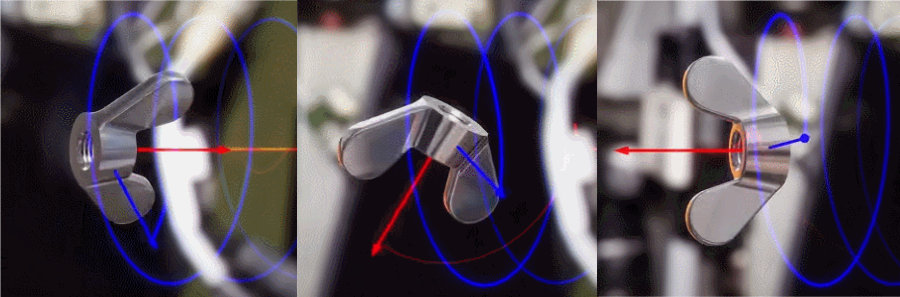
\includegraphics[width=0.9\textwidth]{dzhani.jpg}
\end{center}
   \caption{Una representación del efecto Dzhanibekov \cite{28}.}
\label{fig:10}
\end{figure*}

\begin{figure*}[t]
\begin{center}
\includegraphics[width=1\textwidth]{layers.jpg}
\end{center}
   \caption{Representación de los procesos internos de la Tierra que llevan al cambio ECDO \cite{129}.}
\label{fig:11}
\end{figure*}

\begin{figure}[t]
\begin{center}
   \includegraphics[width=1\linewidth]{llvp.jpg}
\end{center}
   \caption{Una visualización detallada de la LLVP bajo Sudáfrica \cite{28}.}
\label{fig:12}
\label{fig:onecol}
\end{figure}

El principio detrás de un cambio rápido en el eje de rotación de la Tierra reside en la física de los objetos en rotación. El ejemplo canónico de esto es el efecto Dzhanibekov, descubierto por el astronauta ruso Vladimir Dzhanibekov \cite{37}, y representado en la Figura \ref{fig:10}. Un objeto que no está girando perfectamente sobre uno de sus tres ejes principales de inercia no mantendrá un eje de rotación fijo. Si está girando cerca de su segundo eje principal, experimentará lo que parecen ser cambios repentinos en la rotación. Aunque esto no es exactamente lo que creemos que ocurre durante los giros rápidos de la Tierra, el punto es que en ausencia de fuerzas externas, solo la física de rotación puede explicar un cambio rápido en el eje de rotación de la Tierra.

Para ser precisos, la Tierra casi con certeza no experimenta un simple y uniforme efecto Dzhanibekov. Si este fuera el caso, podríamos detectar un cambio gradual en el eje de rotación de la Tierra a lo largo del tiempo. Más bien, creemos que la Tierra experimenta alteraciones periódicas y repentinas en su estructura física, lo que lleva a un desacoplamiento de sus "cuerpos de rotación externa" (corteza/manto) y "cuerpos de rotación internos" (núcleo). Sin una entrada externa, la ley de conservación del momento angular establece que la Tierra no puede cambiar repentinamente su eje de rotación, por lo que un desacoplamiento de los cuerpos de rotación externa e interna es una de las pocas cosas, aparte de un impacto externo en la Tierra, que podría causar un giro repentino y abrupto.
El proceso específico que impulsa la disrupción interna en la Tierra se cree que es un cambio de estado en la estructura del hierro que compone el núcleo de la Tierra (Figura \ref{fig:11}). El núcleo interno está compuesto por hierro (Fe) empaquetado hexagonalmente compacto \cite{141}. A medida que este hcp-Fe se convierte en un estado metálico líquido, libera energía cinética y es arrojado al núcleo exterior. Este cambio de fase reduce la permeabilidad magnética del núcleo, debilitando el campo geomagnético, y libera calor, creando estructuras LLVP (provincias de alto cizallamiento de baja velocidad grandes) (Figura \ref{fig:12}) \cite{38} en el manto, y calentando la superficie de la Tierra a través de los océanos abisales. Ambas tendencias han sido bien documentadas en siglos recientes y se discuten más adelante en este documento.

Se cree que este mismo proceso dentro de la Tierra, ocurriendo de manera inversa, también impulsa el retorno al estado rotacional actual de la Tierra relativamente pronto después de que ocurre el cambio.

\section{Evidencia de un Próximo Cambio de la Tierra}

Existe una fuerte razón para creer que estamos al borde de otro cambio de la Tierra. No ha ocurrido un cataclismo durante varios milenios, lo cual es aproximadamente la frecuencia con la que estos eventos parecen suceder basados en relatos históricos y datos. Los datos más fuertes que apoyan un cambio inminente provienen de datos geomagnéticos recientes, que indican que el campo geomagnético de la Tierra ha estado debilitándose durante aproximadamente dos mil años. Este debilitamiento ha estado acelerándose y ha alcanzado tasas alarmantes en las últimas décadas.

\begin{figure}[t]
\begin{center}
   \includegraphics[width=1\linewidth]{npw.jpg}
\end{center}
   \caption{La posición del polo norte geomagnético de 1590 a 2025, representada en incrementos de 5 años \cite{142}.}
\label{fig:13}
\label{fig:onecol}
\end{figure}


Representado en la Figura \ref{fig:14} está el campo geomagnético de la Tierra en 1590 y 2025 \cite{125,126}. Como se muestra en la figura, el campo se ha debilitado significativamente.

Otra métrica para el debilitamiento del campo geomagnético es la posición del polo norte geomagnético (Figura \ref{fig:13}). Históricamente, el norte geomagnético ha estado ubicado en el Ártico canadiense. Sin embargo, ha estado vagando lentamente durante los últimos siglos y se aceleró significativamente hace algunas décadas. Ahora se está moviendo rápidamente hacia Rusia a una tasa de 55 kilómetros por año \cite{124}.

\begin{figure*}[t]
\begin{center}
\includegraphics[width=0.9\textwidth]{saa.jpg}
\end{center}
   \caption{Una representación del debilitamiento del campo geomagnético de 1590 a 2025. Calculado usando los modelos gufm1 e IGRF-14 \cite{125,126}.}
\label{fig:14}
\end{figure*}

\begin{figure}[t]
\begin{center}
   \includegraphics[width=1\linewidth]{ocean-highlight.jpg}
\end{center}
   \caption{Tasas de calentamiento oceánico profundo ($>$2000 m de profundidad) de 1991 a 2010, circulado en rojo \cite{132}.}
\label{fig:15}
\label{fig:onecol}
\end{figure}

Se cree que el campo magnético de la Tierra es generado por un dínamo interno: columnas circulares de corrientes de magma moviéndose en el núcleo externo de la Tierra debido a su rotación \cite{123}. Un campo geomagnético debilitado es un síntoma de disrupciones en lo profundo de la Tierra. Según la teoría ECDO, estas disrupciones expulsan calor y eventualmente llevan al desacople del manto y el núcleo, causando un cambio de la Tierra \cite{1}.
Hay datos considerables que corroboran la presencia de procesos exotérmicos en el interior de la Tierra. Un calentamiento de la Tierra está documentado en el aumento de las temperaturas superficiales continentales y oceánicas \cite{127,128}, el incremento en los niveles de CO2 atmosférico moviéndose en sincronía con las plumas de calor de la Tierra \cite{129,130}, y una disminución en la extensión global del hielo marino \cite{131}. Los datos sugieren que el aumento de los niveles de CO2 y las temperaturas no son la causa del cambio climático "creado por el hombre", sino más bien efectos aguas abajo de un núcleo exotérmico \cite{129}.

Más significativamente, estudios de las tasas de calentamiento en el océano profundo (profundidades $>$2000 metros) muestran que no solo se están calentando los océanos profundos, sino que las tasas más fuertes de calentamiento se encuentran en la capa abisal (4000 - 6000 m). Este calentamiento de las profundidades marinas tiene un centroide por debajo de 4000 metros \cite{132,129}, lo cual no sería posible si los océanos fueran calentados desde arriba por la atmósfera. Tales datos proporcionan un fuerte apoyo al caso de que los recientes cambios climáticos y geomagnéticos son impulsados ​​por procesos en el interior profundo de la Tierra. La Figura \ref{fig:15} representa las tasas de calentamiento global del océano profundo desde 1991 hasta 2010 \cite{132}.

\section{Modelando el Inminente Cambio de la Tierra}

\begin{figure}[t]
\begin{center}
   \includegraphics[width=1\linewidth]{saa-crop.jpeg}
\end{center}
   \caption{Un cálculo de punto de inflexión basado en la Anomalía del Atlántico Sur apunta a una fecha del 13 de marzo de 2059 \cite{125,126}.}
\label{fig:16}
\label{fig:onecol}
\end{figure}

Predecir el momento del próximo cambio de la Tierra es una tarea compleja. Actualmente, el mejor modelo que tenemos para esto reside en el campo geomagnético de la Tierra: la Anomalía del Atlántico Sur (AAS). Esta región sobre el Atlántico Sur tiene la mayor debilidad en la fuerza del campo geomagnético y se define como el área con una fuerza de campo por debajo de los 32,000 nanotelsas \cite{135}, que fue el valor de campo más débil en 1590. El área de superficie de la Anomalía del Atlántico Sur aumentó del 1% de la superficie de la Tierra en 1590 al 21% en 2025 \cite{136}.

Para obtener una estimación de cuándo podría ocurrir el cambio de la Tierra, ajusté los datos de la extensión de la superficie de la AAS a una ecuación de punto de inflexión de ley de potencia, que modela un sistema complejo acercándose a una transición crítica, en la cual el sistema experimenta un cambio dramático y abrupto. Mis cálculos arrojaron una fecha de punto de inflexión predicha para el 13 de marzo de 2059 (Figura \ref{fig:16}). Esta predicción se volvería más y más precisa a medida que nos acercamos a la transición \cite{136}.

Otras métricas como el desplazamiento del eje de rotación, las anomalías climáticas y los datos sísmicos y volcánicos también pueden ayudarnos a obtener una mejor predicción de cuándo puede ocurrir el próximo cambio de la Tierra.

\section{Cronología Histórica del ECDO}

Si bien es difícil establecer una cronología exacta para eventos pasados de ECDO, parece que hubo al menos 2 eventos de ECDO durante el Holoceno. Nótese el relato contado por Heródoto de sacerdotes egipcios que, \textit{"desde el primer rey hasta este sacerdote de Hefesto que reinó por última vez, hubo trescientas cuarenta y una generaciones de hombres... En este tiempo dijeron que el sol se había movido cuatro veces de su lugar acostumbrado de salida, y donde ahora se pone desde allí había tenido dos veces su salida, y en el lugar de donde ahora sale había tenido dos veces su puesta"} \cite{32}. Platón, que vivió durante el siglo V a.C. \cite{111}, afirmó que después del diluvio que ahogó a Atlántida en un solo día y noche hace 9,000 años, \textit{"ha habido desde entonces muchas inundaciones, y el remanente que sobrevivió en las montañas desconocía el arte de la escritura, y durante muchas generaciones se dedicaron completamente a adquirir los medios de vida"} \cite{112}, lo que sugiere que hubo más de dos cambios desde el final del Younger Dryas circa 9700 a.C. La evidencia física cubierta a lo largo de este documento y en mi investigación \cite{2} proporciona amplia evidencia para el relato de Platón.

La fecha candidata más reciente para un cambio de ECDO es durante el período de 2300 a 1600 A.C., a la que se han datado muchos relatos de inundaciones cataclísmicas (Gun-Yu \cite{113,114,115}, Ogyges \cite{116,117}, Perú \cite{118,119}, Éxodo \cite{120}), destrucciones y abandonos de civilizaciones (Mohenjo-Daro \cite{121}, Creta Minoica\cite{100,101}) y anomalías físicas (eventos de Bond \cite{122}, evento de 4.2 mil años \cite{90}). No hay una amplia convergencia de evidencia más reciente que sugiera un evento catastrófico importante.

\section{Conclusión}

La Operación NANOOK fue un esfuerzo de reconocimiento de la Guerra Fría de los Estados Unidos para mapear el Ártico y la costa norte soviética después de la Segunda Guerra Mundial \cite{137}. Durante su investigación, descubrieron que el polo magnético estaba entre 125 a 200 millas al norte de donde se suponía que debía estar basado en hallazgos de expediciones anteriores. En consecuencia, \textit{"Entre los científicos del gobierno, surgió la pregunta de qué sucedería cuando los polos magnético y geográfico coincidieran. Para responder a esto, bajo el control del proyecto del Dr. Paul A. Siple, se contrató a la Corporación Rand para llevar a cabo estudios de laboratorio utilizando modelos de la tierra construidos con esferas concéntricas: una esfera interna que representa el núcleo de hierro fundido electromagnéticamente cargado de la tierra cuyo eje definía los polos “magnéticos”; y una esfera externa que representa la corteza de la tierra que giraba alrededor de un eje polar “geográfico”. Se determinó a través de repetidos experimentos que a medida que el polo “magnético” se acercaba al polo “geográfico”, el polo “magnético” aceleraría en algún punto su tasa de convergencia como si fuera atraído hacia el polo “geográfico” por una fuerza centrípeta y saltaría para coincidir; pero en lugar de que los polos coincidieran, el polo “magnético” daría rápidamente un “vuelco” alrededor del polo “geográfico”, luego giraría hacia el ecuador como si lo hiciera por fuerza centrífuga, terminando en una posición donde los dos ejes asumieron una divergencia aproximada de 89 grados. Después de que ocurriera este “vuelco” polar, los ejes comenzarían gradualmente a reconverger durante un largo período de tiempo"} \cite{138,139}.

Subsecuentemente, \textit{"En una de las reuniones científicas a las que asistió el Mayor White en el Pentágono a principios de 1948, los científicos discutieron la conveniencia de alertar al público sobre el fenómeno pendiente del vuelco polar. Ninguno de los científicos aceptaría retener la información del público; pero, por otro lado, tampoco llegaron a un acuerdo sobre cómo comunicarlo. El conocimiento de este fenómeno, sintieron algunos, podría por sí mismo destruir la fibra moral de la sociedad. Sus temores parecieron infundados cuando, a principios de la década de 1950, la información sobre el fenómeno del vuelco fue publicada tanto en una columna de periódico como en un artículo de revista, pero sorprendentemente no generó respuestas de parte de un público aparentemente atónito, parroquial o incrédulo"} \cite{138,139}.

¿Por qué no estamos prestando atención a esto? Existe una amplia razón para creer que la Tierra ha dado un vuelco antes. Este documento, junto con la segunda parte del mismo, proporciona un resumen denso de una gran convergencia de evidencias de muchas áreas que sugieren que esto es así, tales como historias de inundaciones en todo el mundo, sal y fósiles marinos cubriendo los continentes, antiguos refugios subterráneos, restos de animales y paisajes geológicos cataclísmicos. Se supone que los humanos tienen cientos de miles de años de antigüedad, sin embargo, la historia moderna solo se remonta a varios miles de años. ¿No podría ser el caso de que de vez en cuando la Tierra da un vuelco, los continentes se limpian y nos vemos obligados a regresar al punto de partida: la Edad de Piedra, reduciendo nuestros registros de historia antigua a un puñado de historias cataclísmicas? Si es así, entonces prevenir que esto ocurra nuevamente podría ser una de las tareas más importantes de la humanidad.

En conclusión, les dejaré con este relato contado en el Timeo, escrito por Platón, sobre una conversación entre Solón, un político ateniense, y sacerdotes egipcios \cite{140}: \textit{"Y en una ocasión, cuando [Solón] deseaba inducirles a hablar sobre la historia antigua, intentó contarles las tradiciones más antiguas de nuestro pueblo, sobre Foroneo, que se decía que fue el primer hombre, y Níobe; y pasó a relatar la leyenda sobre Deucalión y Pirra después del Diluvio, y cómo sobrevivieron a él, y a dar la genealogía de sus descendientes; y al contar el número de años ocupados por los eventos mencionados intentó calcular los períodos de tiempo. Donde uno de los sacerdotes, un hombre tremendamente viejo, le dijo: “Oh Solón, Solón, ustedes los griegos siempre son niños: no existe algo como un griego anciano.” Y al escuchar esto, preguntó: “¿Qué quieres decir con esto?” Y el sacerdote respondió: “Son jóvenes de alma, todos ustedes. Porque en ella no poseen ninguna creencia que sea antigua y derivada de una vieja tradición, ni tampoco una ciencia que sea canosa con la edad. Y esta es la causa de ello: ha habido y habrá muchas y diversas destrucciones de la humanidad, de las cuales las mayores son por fuego y agua, y las menores por innumerables otros medios. En verdad, la historia que se cuenta en su país así como en el nuestro, de cómo en el pasado Faetón, hijo de Helios, unció el carro de su padre, y, porque no pudo conducirlo por la ruta tomada por su padre, quemó todo lo que estaba sobre la tierra y él mismo pereció por un rayo, esa historia, tal como se cuenta, tiene la apariencia de una leyenda, pero la verdad radica en la ocurrencia de un desplazamiento de los cuerpos en los cielos que giran alrededor de la tierra, y una destrucción de las cosas en la tierra por fuego feroz, que se repite a intervalos largos. En tales tiempos, todos aquellos que habitan en las montañas y en lugares altos y secos sufren más destrucción que aquellos que habitan cerca de ríos o del mar; y en nuestro caso el Nilo, nuestro Salvador en otros aspectos, también nos salva en tales momentos de esta calamidad al elevarse. Y cuando, por otro lado, los dioses purgan la tierra con un diluvio de aguas, todos los pastores y cuidadores de ganado que están en las montañas se salvan, pero aquellos en las ciudades de su tierra son arrastrados al mar por los torrentes; mientras que en nuestro país ni entonces ni en ningún otro momento el agua vierte sobre nuestros campos desde arriba, por el contrario, toda tiende naturalmente a brotar desde abajo. De ahí que, por estas razones, lo que aquí se preserva se considera ser lo más antiguo; la verdad es que en todo lugar donde no hay un calor o frío excesivo para impedirlo siempre existe alguna población humana, ahora más, ahora menos en número. Y si algún evento ha ocurrido que es noble o grande o de alguna manera conspicuo, ya sea en su país o en el nuestro o en algún otro lugar del cual sabemos por informe, todos esos eventos se han registrado desde antaño y se han preservado aquí en nuestros templos; mientras que su pueblo y los otros no están más que recién provistos, cada vez, con letras y todas las artes que requieren los Estados civilizados, y cuando, después del usual intervalo de años, como una plaga, el diluvio del cielo cae de nuevo sobre su gente, no deja a ninguno de ustedes salvo a los iletrados e incultos, de modo que se vuelven jóvenes como siempre, sin conocimiento de todo lo que sucedió en tiempos antiguos en esta tierra o en la suya. Ciertamente las genealogías que relataste hace un momento, Solón, sobre la gente de su país son poco más que cuentos de niños; porque, en primer lugar, recuerdan solo un diluvio, aunque muchos ocurrieron previamente; y además, ignoran el hecho de que la raza más noble y perfecta entre los hombres nació en la tierra donde ahora habitan, y de ellos tanto usted mismo desciende como toda su ciudad existente, de alguna pequeña semilla que tuvo la suerte de haber quedado; pero esto ha pasado desapercibido para ustedes porque durante muchas generaciones los sobrevivientes murieron sin tener la capacidad de expresarse por escrito. En verdad, en un momento, Solón, antes de la mayor destrucción por agua, lo que ahora es el Estado ateniense era el más valiente en la guerra y extremadamente bien organizado también en todos los demás aspectos. Se dice que poseía las obras de arte más espléndidas y la política más noble de cualquier nación bajo el cielo de la que hemos oído hablar”}.
Estos mismos sacerdotes, por supuesto, también le contaron a Solón sobre la antigua civilización de la Atlántida: \textit{"Porque todo lo que tenemos aquí, yaciendo dentro de la boca de la que hablamos, es evidentemente un refugio con una entrada estrecha; pero aquello de allá es un verdadero océano, y la tierra que lo rodea puede ser llamada, en el sentido más pleno y verdadero, un continente. Ahora bien, en esta isla de la Atlántida existía una confederación de reyes, de gran y maravilloso poder, que dominaba toda la isla, y muchas otras islas también y partes del continente; y, además, de las tierras aquí dentro de los Estrechos gobernaron Libia hasta Egipto, y sobre Europa hasta Tirrenia. Así que este ejército, estando todo reunido, intentó una vez esclavizar con un solo ataque tanto tu país como el nuestro y todo el territorio dentro de los Estrechos. Y entonces fue, Solón, que la valentía de tu Estado se mostró conspicua por valor y poder a la vista de todo el mundo. Porque se destacó por encima de todos en gallardía y todas las artes bélicas, y actuando en parte como líder de los griegos, y en parte permaneciendo solo por sí mismo cuando fue abandonado por todos los demás, después de enfrentarse a los peligros más mortales, derrotó a los invasores y levantó un trofeo; por el cual salvó de la esclavitud a los que aún no estaban esclavizados, y al resto de nosotros que habitamos dentro de los límites de Hércules los liberó sin reservas. Pero en un tiempo posterior ocurrieron terremotos portentosos e inundaciones, y un día y noche lamentables les sobrevinieron, cuando todo el cuerpo de tus guerreros fue tragado por la tierra, y la isla de la Atlántida asimismo fue tragada por el mar y desapareció"}.

\section{Agradecimientos}

Gracias a Ethical Skeptic, el autor original de la tesis ECDO, por completar su innovadora y reveladora tesis y compartirla con el mundo. Su tesis tripartita \cite{1} sigue siendo el trabajo seminal para la teoría de la Oscilación de Como Desacoplamiento de Núcleo-Manto Exotérmico (ECDO), y contiene mucha más información sobre el tema de la que he cubierto brevemente aquí.

Gracias a Ankit, quien procesó los datos de recopilación de cataclismos en la Tabla 1.

Muchas gracias a PS por revisar este documento.

Y, por supuesto, gracias a los gigantes sobre cuyos hombros nos apoyamos; aquellos que han realizado toda la investigación e indagación que hicieron posible este trabajo y se esforzaron por traer luz a la humanidad.

\clearpage
\twocolumn

\section{Imágenes Adicionales}

\begin{figure}[H]
\begin{center}
   \includegraphics[width=1\linewidth]{wave.jpg}
\end{center}
   \caption{Una mirada de cerca a la erosión de onda parabólica en la pirámide de Kefrén \cite{27}.}
\label{fig:19}
\label{fig:onecol}
\end{figure}

\begin{figure}[H]
\begin{center}
   \includegraphics[width=1\linewidth]{star-stone.jpg}
\end{center}
   \caption{El mapa de estrellas tallado en piedra en uno de los ejes de la pirámide de Keops \cite{28}.}
\label{fig:20}
\label{fig:onecol}
\end{figure}

\begin{figure*}[t]
\begin{center}
\includegraphics[width=1\textwidth]{deepsea.jpg}
\end{center}
   \caption{Una visualización de la anomalía de calentamiento en los océanos profundos y abisales en comparación con una curva normal de calentamiento del océano atmosférico. La anomalía de calentamiento general ha sido tomada de NOAA \cite{147}, las distribuciones de calentamiento profundo y abisal de un estudio de Desbruyeres \cite{132}, y el procesamiento de datos y visualización por Ethical Skeptic \cite{129}.}
\label{fig:21}
\end{figure*}

\begin{figure*}[t]
\begin{center}
\includegraphics[width=1\textwidth]{sealevel.jpeg}
\end{center}
   \caption{El nivel del mar muestra un aumento del 20\% en la varianza durante 75 años a través de 63 estaciones, lo que indica un aumento en la velocidad de la corriente. Los aumentos en la varianza del nivel del mar son concurrentes con los pulsos de calor en el océano, indicando que ambos pueden ser causados por el calentamiento desde las profundidades debajo de los océanos de la Tierra \cite{2,129}.}
\label{fig:22}
\end{figure*}
\begin{figure*}[t]
\begin{center}
\includegraphics[width=1\textwidth]{co2.jpg}
\end{center}
   \caption{El CO2 atmosférico en ppm ha aumentado de manera consistente en los últimos 45 años, probablemente causado por un aumento en las temperaturas oceánicas. Fuente: NOAA \cite{148,129}.}
\label{fig:23}
\end{figure*}

\begin{figure*}[t]
\begin{center}
\includegraphics[width=1\textwidth]{ice.jpg}
\end{center}
   \caption{La extensión del hielo marino global se ha reducido en los últimos 45 años, debido a un calentamiento de la Tierra. Fuente: ADS \cite{149}.}
\label{fig:24}
\end{figure*}

\clearpage
\twocolumn

{\small
\bibliographystyle{ieee}
\bibliography{egbib}
}

\end{document}
